%auto-ignore
\documentclass[tikz]{standalone}

\begin{document}
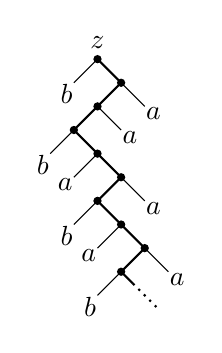
\begin{tikzpicture}[scale=0.3]

\draw [thick] (0,0) node [above] {$z$} -- (1,-1) -- (-1,-3) --
++(2,-2) -- ++(-1,-1) --
++(2,-2) -- ++(-1,-1) --
++(0.5,-0.5);

%\foreach \x in {-1,0,1,2,3} {
%	\draw (\x,-2-\x) to +(-1,-1) node [below left] {$a$};
%	\fill (\x,-2-\x) circle (2pt);
%}

\draw (0,0) to +(-1,-1) node [below left=-0.3em] {$b$};
\draw (-1,-3) to +(-1,-1) node [below left=-0.3em] {$b$};
\draw (0,-6) to +(-1,-1) node [below left=-0.3em] {$b$};
\draw (1,-9) to +(-1,-1) node [below left=-0.3em] {$b$};

\draw (0,-4) to +(-1,-1) node [below left=-0.3em] {$a$};
\draw (1,-7) to +(-1,-1) node [below left=-0.3em] {$a$};

\draw (1,-1) to +(1,-1) node [below right=-0.3em] {$a$};
\draw (0,-2) to +(1,-1) node [below right=-0.3em] {$a$};
\draw (1,-5) to +(1,-1) node [below right=-0.3em] {$a$};
\draw (2,-8) to +(1,-1) node [below right=-0.3em] {$a$};

\draw [dotted,thick] (1.5,-9.5) to +(1,-1);

\foreach \x in {
	(0,0),
	(1,-1),
	(0,-2),
	(-1,-3),
	(0,-4),
	(1,-5),
	(0,-6),
	(1,-7),
	(2,-8),
	(1,-9)
} {
	\fill \x circle (5pt);
}

\end{tikzpicture}
\end{document}